\chapter{Teorie}
\label{2-teorie}

Nejdůležitějšími prvky dronu jsou motory s vrtulemi, řídící jednotka a IMU. Motory s vrtulemi fungují jako ventilátory, které ženou vzduch určitým směrem, pokud všechny motory ženou vzduch proti zemi, dron by měl vzlétnout. Proč je tedy potřeba řídící jednotka a IMU? Bohužel rozložení hmotnosti dronu a drobné mechanické rozdíly v motorech zapříčiní různé tahy jednotlivých motorů. Díky ovládání motorů podle řídící jednotky, dokážeme vliv různých tahů vyrovnat a dron může létat.\\
Jakým způsobem vykonává dron pohyb? Let dronu v určitém směru je způsoben snížením výkonu motorů ve směru letu a zvýšením výkonu motorů v opačném směru letu, viz obrázek č. 3.1. Rotace dronu je uskutečněna zvýšením výkonu motorů s různými typy vrtulí, po směru hodinových ručiček a proti (CW a CCW orientace). Zvýšením výkonu na motorech s vrtulemi s orientací CW se dron otáčí po směru hodinových ručiček, s orientací CCW proti směru hodinových ručiček, viz obrázek 3.2.\\
%https://www.wired.com/2017/05/the-physics-of-drones/

\begin{figure}[H]
	\centering
	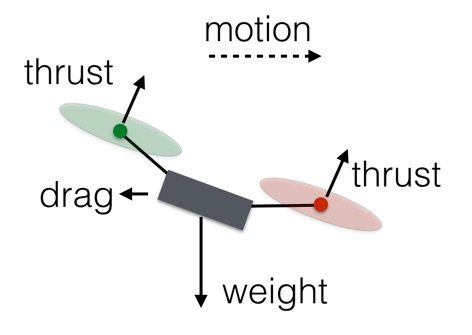
\includegraphics[width=7cm]{pictures/dronfly.jpg}
	\caption{Let určitým směrem(motion-směr, thrust/drag-tah, weigth-váha)}
	\cite{physicdrone}
\end{figure}
%https://devusa.djicdn.com/images/flightController-concepts/altitude-7e757661b6.png

\begin{figure}[H]
	\centering
	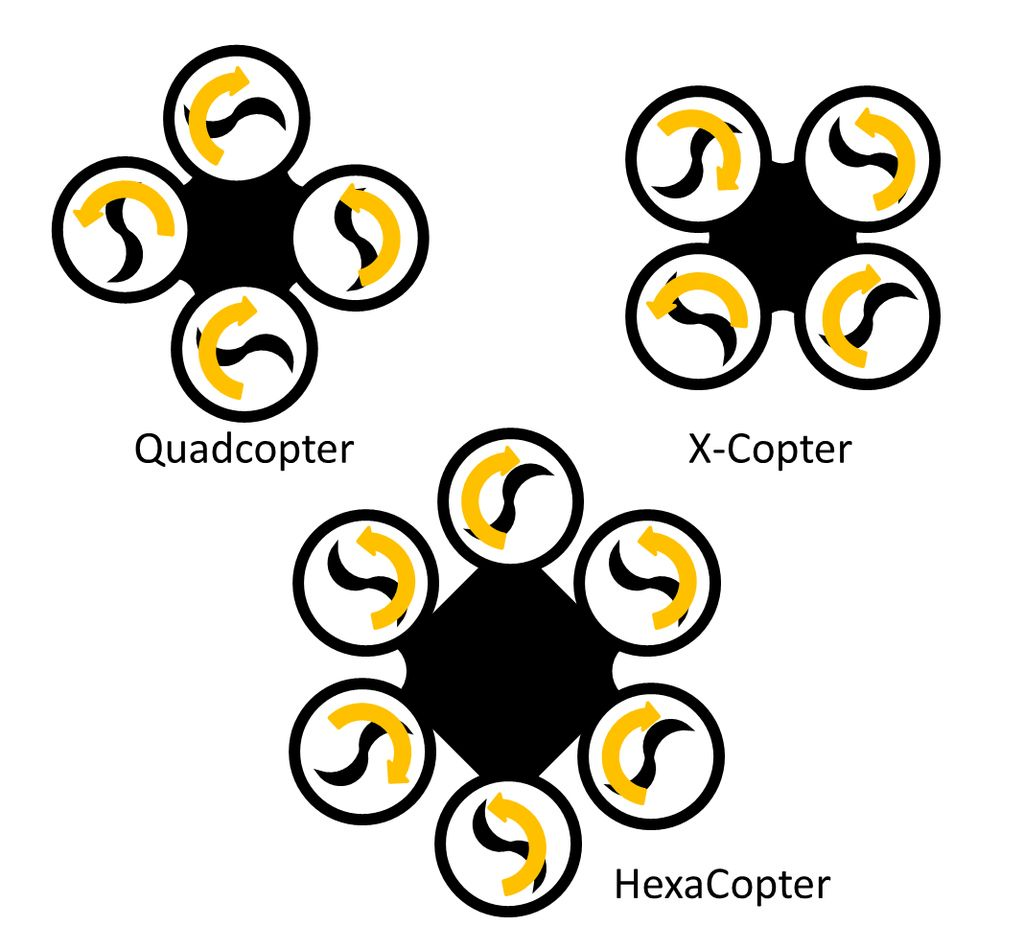
\includegraphics[width=10cm]{pictures/dronrot.png}
	\caption{Přehled vtrulí se CW a CCW orientací}
	\cite{rotdrone}
\end{figure} 
Důležitou roli při letu dronu hraje IMU jednotka, která určuje úhly rotace. Roll je úhel rotace kolem osy X, pitch je úhel rotace kolem osy Y a yaw je úhel rotace kolem osy Z. Souřadný systém má střed v težišti dronu. Osa X směřuje do směru letu, osa Y je na ni kolmá a osa Z je totožná s tížnicí, viz obrázek 3.3.\\
Řízení dronu probíhá přes jmenované úhly pitch, roll a yaw. Uživatel zadává úhly a mikrokprocesor podle IMU zadané úhly nastavuje. Nastavení úhlu vzniká pomocí zvyšování a snižování výkonu na jednotlivých motorech. Popis řízení dronu je podrobněji vysvětlen v kapitole Ovládání jednotlivých elektronických částí u Letového kontroléru.\\
Existuje vícero překladů úhlů pitch, roll a yaw (např. vybočení, klonění a  klopení, nebo příčný náklon, podélný sklon a zatáčení), pro zjednodušení bude v textu ponecháno pojmenování v anglickém jazyce.\\
%Source: https://www.instructables.com/id/Design-Build-and-Improve-a-Quadcopter/

\begin{figure}[H]
	\centering
	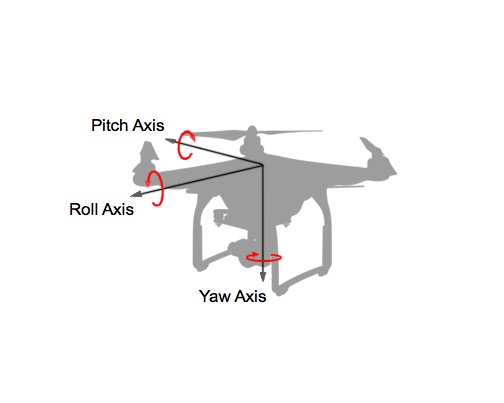
\includegraphics[width=10cm]{pictures/rotangle.png}
	\caption{Úhly rotace (Axis - Osa)}
	\cite{diffdrone}
\end{figure} 
